\chapter{Results}
\label{ch:results}

In this chapter we cover results from both the Machine Learning (Section~\ref{sec:results_machine_learning}) and Background Subtraction (Section~\ref{sec:results_background_subtraction}) methods. Results in each section include a summary tools used to collect data, the size of the analyzed data, and a discussion on the effectiveness of each technique.

\section{Feature Detection and Machine Learning}
\label{sec:results_machine_learning}

Approximately 500 computers processed more than 63 million images for the Wildlife@Home SVM classification project. More than 3,500 work units have been successfully processed by volunteers with Linux, OSX, and Windows computers and have collected SURF descriptors for more than 1,750 hours of wildlife video. Most work units process a single hour long video recorded at 10 frames per second. Each work unit typically takes 3 hours of CPU time depending on video length, the number of descriptors being handled, and processor speed. Depending on SURF parameters and video content each work unit returns roughly 2,000 descriptors for each event type in the video. These descriptors are stored for SVM training and testing.

For testing results, a variety of parameters were chosen for SVM training with LIBSVM\@. Initial parameters were determined by the LIBSVM grid search program, \emph{grid.py}. All tested results fall in the ranges below:

\begin{align}
\gamma =&~\text{\numrange{0.5}{10.0}} \nonumber \\
c =&~\text{\numrange{0.5}{10.0}} \nonumber \\
w_{-1} =&~\text{\numrange{0.5}{50.0}} \nonumber \\
w_{+1} =&~\text{\numrange{0.5}{50.0}} \nonumber
\label{eq:svm_parameters}
\end{align}

Descriptors were collected for sharp-tailed grouse, interior least tern, and piping plover. For each species 5 different SURF minimum hessian values were sampled, 100, 150, 200, 300, and 500. The hessian value controls the threshold for a Hessian corner detection algorithm used in SURF for determining which points in the image to use a possible point of interest. The lower the minimum hessian threshold value the larger the number of descriptors collected from each frame.

\subsection{Video Identification Results}
\label{sec:inital_test}

We selectively chose a single tern nest for testing as there is less background noise and fewer descriptors collected from the video background. Since many videos have dramatic lighting changes and indistinguishable objects at night we removed nighttime footage and videos with dramatic shadow changes from sun orientation. These videos greatly skew results from the feature detection algorithms which focus on edge and corner detection. Upon removal of these videos from our selected tern nest we have 24 acceptable videos remaining for SVM training. These videos contain 25,000 positive and 23,000 negative descriptors. Three methods could be used to provide data to the SVM\@. Method 1 is to train on all 47,000 of the descriptors. Method 2, subtract the negative features from the positive features and accept only those outside of a threshold for training. This reduces the positive set size to 120 descriptors. Method 3, manually select the nest location with a bounding box and use the descriptors on the nest as the positive training set resulting in a positive set of about 8000 descriptors. Method 1 is the slowest and hardest to train because of the volume of features along with the large overlap in positive and negative features. Option 2 is easiest to train and theoretically the most accurate however the difficulty comes in choosing the descriptor subtraction threshold. Too large of threshold leads to training on video outliers such as video artifacts and too large a threshold will continue to have similar problems as Method 1. Method 3 can work well but requires manual selection of the nest location and will not work if the bird is not always directly on the nest. We used method 3 in our system to reduce the system memory footprint and SVM training time, reduce the chance of a possible event classification error, and to test the algorithms in the best possible scenario. A classification could happen when an expert marks \emph{bird not in video} when the bird has just appeared or possibly quickly entered and exited the camera view. This type of error will cause SURF to misclassify the extracted features from the incorrectly marked frames and feed incorrect data to the SVM\@.

Results for this sample data using method 3 can be seen in figures~\ref{fig:begin_test_video} and~\ref{fig:end_test_video}. Keypoints from the video were drawn on each frame and colored according to their SVM classification. The negative SVM classifications are colored red, positive classifications colored green, and the closest matches to training data are colored blue. The green and blue points were redrawn on all successive frames to show a clustering and get an idea of their overall representation. As seen in Figure~\ref{fig:begin_test_video} there is very little correlation in the position of points and the location of the bird but as the video progresses more and more training points start to position themselves on the bird and around the nest in Figure~\ref{fig:end_test_video}. However, since the majority of green points aren't necessarily enclosed in the same region it is likely the SVM is not being optimally trained on the descriptors. This is a sign of overfitting, specifically on any video artifacts that are appearing only in the positively correlated frames such as \emph{parent on nest}. If we saw a larger number of positive classifications than negative classifications it would be a sign of underfitting the data and accepting too many descriptors.

\subsection{Tern Presence Correlation}
\label{sec:tern_correlation}

\begin{figure}
\centering
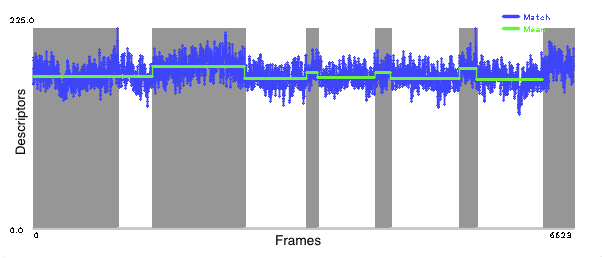
\includegraphics[width=5.5in]{tern_single_video_svm}
\caption{Single tern video descriptors run against itself with training features using method 3 for SVM training. White segments indicate frames where an expert has marked \emph{bird in frame} and gray regions are segments where the expert marked \emph{not in frame}. The blue line indicates the number of descriptors found to match a \emph{bird in frame} event. The green line represents the average number of matched descriptors for its corresponding gray or white time segment.}
\label{fig:tern_single_video}
\end{figure}

\begin{figure}
\centering
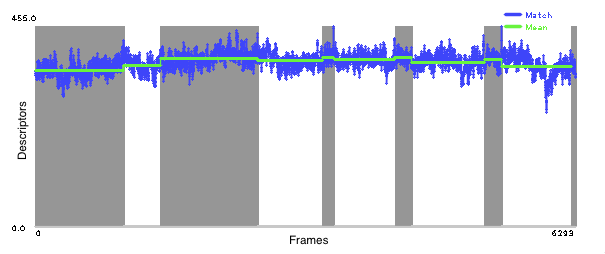
\includegraphics[width=5.5in]{tern_three_video_loo_svm}
\caption{Three tern videos using leave-one-out cross validation and method 3 for SVM training. White segments indicate frames where an expert has marked \emph{bird in frame} and gray regions are segments where the expert marked \emph{not in frame}. The blue line indicates the number of descriptors found to match a \emph{bird in frame} event. The green line represents the average number of matched descriptors for its corresponding gray or white time segment.}
\label{fig:tern_three_video}
\end{figure}

In order to predict bird presence we selected three interior least tern videos from the same nest and charted the number of descriptor matches against the expert classified bird presence events for that video. Results can be seen in Figure~\ref{fig:tern_single_video} and~\ref{fig:tern_three_video} where the gray background indicates bird presence, white background indicates bird absence, the blue line is the number of matching descriptors in each frame, and the green line is the mean for that segment of either bird presence or absence. Figure~\ref{fig:tern_single_video} shows results for a single video's descriptors tested against itself and Figure~\ref{fig:tern_three_video} shows results using descriptors from videos at the same nesting site against the same video used in Figure~\ref{fig:tern_single_video}. As seen in each case there is a signal indicating an increase in matching descriptors when the bird is present and a decrease when the bird is absent. The optimal case in Figure~\ref{fig:tern_single_video} has only a slightly more pronounced signal which indicates descriptors across videos from the same nest have similar values.


\subsection{Effectiveness of Feature Detection and Machine Learning}
\label{sec:results_machine_learning_effectiveness}

Results from this feature detection and machine learning research shows that there may be a slight correlation in the number of SVM matches and bird presence in a video. This however is not a good indication since we have only trained and tested on the best possible scenarios and still see mixed results (Figures~\ref{fig:tern_single_video} and~\ref{fig:tern_three_video}).

Many factors may be causing the poor performance from the machine learning. Video quality and resolution, random noise detected during intra coded frames from video compression, moving shadows from outdoor video, and a large number of overlapping descriptors from frames with a bird and frames without a bird can all be causes of poor SVM performance. It is likely that many of these factors contribute to the results we see in Figures~\ref{fig:tern_single_video} and~\ref{fig:tern_three_video}.


\section{Background Subtraction}
\label{sec:results_background_subtraction}

The three background subtraction algorithms were run against a set of 105 tern and plover videos and 109 grouse videos. The plover and tern video totals 77.05 hours, and the grouse video totals 205.39 hours. Video lengths range anywhere from 30 minutes to 2 hours in length. Each algorithm runs at more than 10 frames per second (the recording frame rate) on a hyperthreaded 3.5 GHz core and is considered capable of real-time processing. Results were collected using a Mac Pro and 12 logical cores, which took approximately 48 hours. They were compared to many weeks worth of observations made by project expert scientists and volunteer citizen scientists to determine algorithm accuracy.


\subsection{Detecting Events with Background Subtraction}
\label{sec:event_detection}

\begin{table}
\centering
\caption{Algorithm Accuracy vs Expert Scientists on Tern and Plover Nests}
\label{table:algorithm_accuracy_experts}
\begin{tabular}{lrrrr}
    \toprule
    Event Type & Event Count & MOG & ViBe & PBAS\\
    \midrule
    Preen & 180 & 170 & 138 & 147\\
    Scratch & 4 & 4 & 2 & 2\\
    Not In Video & 732 & 632 & 578 & 607\\
    Nest Exchange & 22 & 16 & 16 & 16\\
    Foraging & 82 & 71 & 52 & 56\\
    Adult-to-Adult Feed & 20 & 6 & 6 & 6\\
    Nest Defense & 4 & 4 & 4 & 4\\
    Predator & 12 & 10 & 7 & 9\\
    Non-Predator Animal & 22 & 16 & 15 & 15\\
    Unspecified & 350 & 93 & 66 & 78\\
    On Nest & 932 & 665 & 582 & 608\\
    Off Nest & 2312 & 1960 & 1775 & 1876\\
    \bottomrule
\end{tabular}
\end{table}

\begin{table}
\centering
\caption{Algorithm Accuracy vs Citizen Scientists on Tern and Plover Nests}
\label{table:algorithm_accuracy_users}
\begin{tabular}{lrrrr}
    \toprule
    Event Type & Event Count & MOG & ViBe & PBAS\\
    \midrule
    Not In Video & 82 & 79 & 79 & 79\\
    Nest Exchange & 4 & 2 & 2 & 4\\
    Adult-to-Adult Feed & 14 & 14 & 14 & 14\\
    Non-Predator Animal & 16 & 16 & 14 & 14\\
    Unspecified & 10 & 10 & 10 & 10\\
    On Nest & 140 & 138 & 112 & 112\\
    Off Nest & 146 & 144 & 143 & 143\\
    \bottomrule
\end{tabular}
\end{table}


\begin{table}
\centering
\caption{Algorithm Accuracy vs Expert Scientists on Grouse Nests}
\label{table:algorithm_accuracy_grouse_experts}
\begin{tabular}{lrrrr}
    \toprule
    Event Type & Event Count & MOG & ViBe & PBAS\\
    \midrule
    Not In Video & 284 & 274 & 258 & 270\\
    Eggshell Removal & 6 & 4 & 5 & 5\\
    In Video & 130 & 128 & 129 & 129\\
    Predator & 6 & 5 & 5 & 5\\
    Unspecified & 2 & 2 & 2 & 2\\
    Attack & 2 & 2 & 2 & 2\\
    Physical Inspection & 60 & 52 & 56 & 56\\
    Observation & 44 & 41 & 39 & 41\\
    On Nest & 216 & 196 & 174 & 178\\
    Off Nest & 492 & 470 & 439 & 461\\
    \bottomrule
\end{tabular}
\end{table}

\begin{table}
\centering
\caption{Algorithm Accuracy vs Citizen Scientists on Grouse Nests}
\label{table:algorithm_accuracy_grouse_users}
\begin{tabular}{lrrrr}
    \toprule
    Event Type & Event Count & MOG & ViBe & PBAS\\
    \midrule
    Not In Video & 308 & 298 & 261 & 274\\
    Nest Defense & 2 & 2 & 2 & 2\\
    Predator & 14 & 12 & 10 & 12\\
    Non-Predator Animal & 2 & 2 & 1 & 2\\
    Unspecified & 2 & 0 & 2 & 2\\
    Attack & 22 & 18 & 20 & 21\\
    Physical Inspection & 46 & 46 & 45 & 46\\
    Observation & 8 & 7 & 7 & 8\\
    On Nest & 340 & 317 & 249 & 253\\
    Off Nest & 588 & 576 & 506 & 532\\
    \bottomrule
\end{tabular}
\end{table}

Tables~\ref{table:algorithm_accuracy_experts},~\ref{table:algorithm_accuracy_grouse_experts},~\ref{table:algorithm_accuracy_users}, and~\ref{table:algorithm_accuracy_grouse_users} present how well each algorithm matched up to project scientists and volunteers for sharptailed grouse, and piping plover and least tern combined. Piping plover and least tern results were combined as the birds and environments are highly similar, and both species are being observed for the same set of events. The \emph{Event Count} column shows the total number of each event that occurred in the set of videos analyzed, and the following columns present how many of those events the background subtraction algorithm found.

Any background subtraction detected events that occur within 30 seconds of the start or end time of a scientist observed event are marked as a match. Multiple matches to the same start and end event from the same scientist are ignored. Since all three algorithms are adaptive, learning takes place in each algorithm where it will begin to ignore bird presence and absence on the nest. Event start and end times that take place within the first 10 seconds of the beginning of the videos were ignored as the algorithms did not have time to learn an initial background yet.

\begin{sidewaystable}
\centering
\caption{Algorithm Accuracy with Consensus vs Expert Scientists on Tern and Plover Nests}
\label{table:algorithm_consensus_experts}
\begin{tabular}{lrrrrrr}
    \toprule
    Event Type & Event Count & Any Alg & All Alg & MOG \& ViBe & MOG \& PBAS & ViBe \& PBAS\\
    \midrule
    Preen & 180 & 174 & 137 & 138 & 143 & 137\\
    Scratch & 4 & 4 & 2 & 2 & 2 & 2\\
    Not In Video & 732 & 635 & 576 & 576 & 606 & 576\\
    Nest Exchange & 22 & 16 & 16 & 16 & 16 & 16\\
    Foraging & 82 & 73 & 51 & 52 & 54 & 51\\
    Adult-to-Adult Feed & 20 & 6 & 6 & 6 & 6 & 6\\
    Human & 2 & 0 & 0 & 0 & 0 & 0\\
    Nest Defense & 4 & 4 & 4 & 4 & 4 & 4\\
    Predator & 12 & 11 & 6 & 6 & 8 & 7\\
    Non-Predator Animal & 22 & 19 & 12 & 12 & 14 & 13\\
    Unspecified & 350 & 94 & 66 & 66 & 77 & 66\\
    On Nest & 932 & 669 & 572 & 580 & 606 & 572\\
    Off Nest & 2312 & 1974 & 1763 & 1769 & 1868 & 1763\\
    \bottomrule
\end{tabular}
\end{sidewaystable}

Table~\ref{table:algorithm_consensus_experts} compares results from combining all three background subtraction algorithms. The \emph{Any Alg} column shows the number of events that matched any one of the three algorithms, and the \emph{All Alg} column shows the number of events that matched all three algorithms. Using events marked by any algorithm provided a small increase in events detected over PBAS for all event types, however using a consensus showed a dramatic decrease in the number of events found. This decrease is indicative that the three different algorithms are not finding overly similar areas of activity within the videos.


\subsection{Analysis of False Positives}
\label{sec:false_positives}

\begin{table}
\centering
\caption{Algorithm False Positives vs Expert Scientists}
\label{table:algorithm_false_positives_experts}
\begin{tabular}{lrrrrrr}
    \toprule
    \multicolumn{1}{c}{} &
    \multicolumn{2}{c}{MOG} &
    \multicolumn{2}{c}{ViBe} &
    \multicolumn{2}{c}{PBAS}\\
    \midrule
    \multicolumn{1}{c}{Species} &
    \multicolumn{1}{c}{$\mu$} &
    \multicolumn{1}{c}{$\sigma$} &
    \multicolumn{1}{c}{$\mu$} &
    \multicolumn{1}{c}{$\sigma$} &
    \multicolumn{1}{c}{$\mu$} &
    \multicolumn{1}{c}{$\sigma$}\\
    \midrule
    Grouse & 139.67 & 144.76 & 74.31 & 95.92 & 73.83 & 100.64\\
    Tern & 5.78 & 35.37 & 2.76 & 15.86 & 1.58 & 6.89\\
    Plover & 4 & 7.63 & 0.50 & 1.07 & 0.63 & 1.41\\
    \bottomrule
    \end{tabular}
\end{table}

\begin{table}
\centering
\caption{Algorithm False Positives vs Citizen Scientists}
\label{table:algorithm_false_positives_users}
\begin{tabular}{lrrrrrr}
    \toprule
    \multicolumn{1}{c}{} &
    \multicolumn{2}{c}{MOG} &
    \multicolumn{2}{c}{ViBe} &
    \multicolumn{2}{c}{PBAS}\\
    \midrule
    \multicolumn{1}{c}{Species} &
    \multicolumn{1}{c}{$\mu$} &
    \multicolumn{1}{c}{$\sigma$} &
    \multicolumn{1}{c}{$\mu$} &
    \multicolumn{1}{c}{$\sigma$} &
    \multicolumn{1}{c}{$\mu$} &
    \multicolumn{1}{c}{$\sigma$}\\
    \midrule
    Grouse & 118.27 & 136.17 & 53.14 & 74.65 & 53.90 & 82.10\\
    Tern & 0.41 & 1.74 & 0.22 & 0.80 & 0.15 & 0.46\\
    \bottomrule
\end{tabular}
\end{table}

Tables~\ref{table:algorithm_false_positives_experts} and~\ref{table:algorithm_false_positives_users} provide an analysis of false positives generated by the background subtraction algorithms. False positives were counted by the number of computer classified events that occur during a user classified \emph{Not In Video} event. Results are reported as the mean ($\mu$) and standard deviation ($\sigma$) of false positives during any \emph{Not in Video} event by any scientist over all videos tested for that species. Videos without a \emph{Not In Video} event were ignored to prevent padding the results. A 10 second buffer is used after the start and before the end of the \emph{Not In Video} events to avoid counting edge case movement as a false positive. This was used as a measure for false positives since at any other time a detection may correspond to an unmarked event, such as motion from the bird on the nest.


\subsection{Effectiveness of Background Subtraction}
\label{sec:results_effectiveness}

The initial background subtraction results in Tables~\ref{table:algorithm_accuracy_experts},~\ref{table:algorithm_accuracy_users},~\ref{table:algorithm_accuracy_grouse_experts}, and~\ref{table:algorithm_accuracy_grouse_users} show that background subtraction is accurate enough to be a reliable detection method for this type of video. Especially in the case of the \emph{Not In Video}, \emph{On Nest}, and \emph{Off Nest} events, the detection accuracy is high enough to be useful for decision making. The other event sample sizes are still too small, requiring more results to be collected. MOG has the highest accuracy on both the tern and plover video however we also see the highest false positive rates from MOG across all species types. Due to MOG's high rate of false positives, PBAS is likely the best overall performing algorithm due to its low false positive rate and high accuracy. Utilizing results from any algorithm (Table~\ref{table:algorithm_consensus_experts}) shows a slight improvement over in performance over any individual algorithm. We also see than PBAS has a low number of false positives on the tern and plover observations (Tables~\ref{table:algorithm_false_positives_experts} and~\ref{table:algorithm_false_positives_users}).

The Grouse have the highest average number of false positives (Tables~\ref{table:algorithm_false_positives_experts} and~\ref{table:algorithm_false_positives_users}) and by far the highest standard deviation of false positives. The high variance in the grouse results suggest that some videos may have a low number of false positives, presumably indicating better precision on less windy videos. This also indicates that the high accuracy on the grouse videos (Tables~\ref{table:algorithm_accuracy_grouse_experts} and~\ref{table:algorithm_accuracy_grouse_users}) may not solely be false positives due to moving foliage.

Another major cause for algorithm inaccuracy and large variance in false positives (especially in the Least Tern samples) is from camera lighting autocorrection discussed in Section~\ref{sec:methodology} and seen in Figure~\ref{fig:lighting_example}. Changes in scenery brightness from transitions in time of day or significant overhead cloud movement cause the camera to adjust brightness and can cause large scale false foreground detection. If the camera rapidly and repeatedly changes the brightness we see regions of video that the foreground algorithms cannot adapt to as shown in Figure~\ref{fig:lighting_example}. Due to the nature of PBAS, it adjusts to the rapid brightness changes but this still causes false negatives if a scientist observed event does occur during or shortly after the brightness adjustments.

\begin{sidewaysfigure}[!t]
\centering
\subfloat[Sample I]{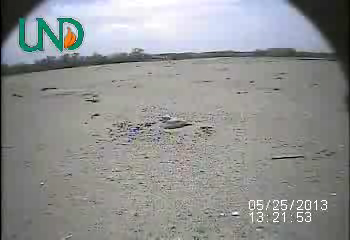
\includegraphics[width=2.9in]{23052_bright}
\label{fig:bight_scene}}
\hfil
\subfloat[Sample II]{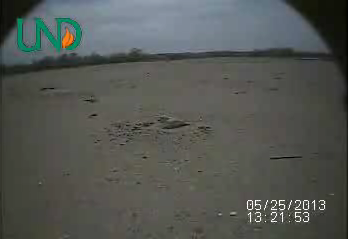
\includegraphics[width=2.9in]{23052_dark}
\label{fig:dark_scene}}
\hfil
\subfloat[Sample Issue Foreground Count]{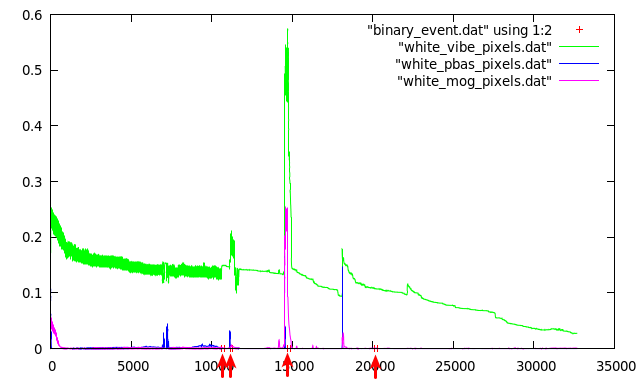
\includegraphics[width=2.9in]{23052_lighting_issue}
\label{fig:lighting_issue}}
\caption{Rapid and repeating brightness adjust caused by overhead cloud movement. Brightness is alternated multiple times per second creating a messy foreground pixel timeline show in Figure~\ref{fig:lighting_issue}. ViBe fails to adapt to the rapid changes and both MOG and PBAS become ignorant to small pixel changes required to detect bird movement.}
\label{fig:lighting_example}
\end{sidewaysfigure}

Other detection errors are caused by video compression noise, and species cryptic coloration. The original archival Wildlife@Home videos taken by the field cameras are compressed by the hardware in part due to storage reasons. With these background subtraction algorithms working on moderate to heavy compression, false positives are caused during transitions between intra coded frames. More sensitive events such as preens and scratches can be difficult to detect due to the small amount of motion involved (typically just body rotation and head movement) given the camera distance, along with the cryptic coloration of the species. With the surrounding area taking on such a similar color to the bird a simple preen or scratch may easily go undetected by a background subtraction algorithm.

It is also worth noting that many detected events may not line up with the start or end time of a scientist observation but may still be a cause of bird motion. For example in Figure~\ref{fig:no_false_positives}, no events occur while the bird is off the nest, but we see sporadic events while it is on the nest. This could be caused by bird adjustment on the nest or unmarked bird grooming events. The frequency of events occurring during a video may also serve as an additional indicator of bird presence, and merits further investigation.

